\subsection{Overall Performance}

\begin{table}[H]
  \centering
  \caption{Test performance across datasets. For regression tasks we report RMSE; for classification tasks we report Accuracy and AUC-ROC.}
  \scriptsize
  \resizebox{\textwidth}{!}{
    \begin{tabular}{lcccc}
      \toprule
      \textbf{Dataset} & \textbf{xRFM} & \textbf{XGBoost} & \textbf{Random Forest} & \textbf{TabPFN} \\
      \midrule
      Abalone (RMSE) & 2.1013 & 2.1737 & 2.1891 & 2.0549 \\
      Diamonds (RMSE) & 520.0493 & 562.1491 & 833.2694 & 519.3203 \\
      Superconductor (RMSE) & 9.8139 & 9.4001 & 10.7205 & 9.1863 \\
      Obesity Level (Acc./AUC) & 0.9835 / 0.9997 & 0.9669 / 0.9990 & 0.9433 / 0.9926 & 0.9929 / 1.0000 \\
      Sleep Health (Acc./AUC) & 0.8905 / 0.9756 & 0.9465 / 0.9909 & 0.8458 / 0.9682 & 0.9435 / 0.9933 \\
      \bottomrule
    \end{tabular}
  }
  \label{tab:overall_performance}
\end{table}

\begin{table}[H]
  \centering
  \caption{Compute cost across datasets: training time and inference time per sample.}
  \scriptsize
  \resizebox{\textwidth}{!}{%
    \begin{tabular}{lcccccccc}
      \toprule
      \textbf{Dataset} &
      \textbf{xRFM Fit (s)} & \textbf{xRFM Inf./Sample (s)} &
      \textbf{XGB Fit (s)} & \textbf{XGB Inf./Sample (s)} &
      \textbf{RF Fit (s)} & \textbf{RF Inf./Sample (s)} &
      \textbf{TabPFN Fit (s)} & \textbf{TabPFN Inf./Sample (s)} \\
      \midrule
      Abalone & 0.4593 & $1.01 \times 10^{-5}$ & 0.1895 & $2.69 \times 10^{-6}$ & 0.0593 & $4.43 \times 10^{-5}$ & 0.9748 & $2.66 \times 10^{-3}$ \\
      Diamonds & 80.3824 & $1.10 \times 10^{-4}$ & 0.4962 & $6.95 \times 10^{-7}$ & 0.1017 & $2.65 \times 10^{-6}$ & 3.6773 & $6.97 \times 10^{-2}$ \\
      Superconductor & 12.8962 & $5.03 \times 10^{-5}$ & 2.0742 & $2.63 \times 10^{-6}$ & 0.2184 & $6.45 \times 10^{-6}$ & 6.4547 & $7.93 \times 10^{-2}$ \\
      Obesity Level & 0.1568 & $7.32 \times 10^{-6}$ & 0.6880 & $6.67 \times 10^{-5}$ & 0.1095 & $6.01 \times 10^{-5}$ & 0.2680 & $1.88 \times 10^{-3}$ \\
      Sleep Health & 11.6116 & $4.97 \times 10^{-5}$ & 1.4002 & $4.75 \times 10^{-6}$ & 0.1477 & $6.56 \times 10^{-6}$ & 1.7053 & $1.06 \times 10^{-2}$ \\
      \bottomrule
    \end{tabular}%
  }
  \label{tab:compute_cost}
\end{table}

Overall, XGBoost and TabPFN deliver strong predictive performance across both regression and classification tasks (Table~\ref{tab:overall_performance}). xRFM is competitive on several datasets, but its training time can be substantially higher on larger problems (e.g., Diamonds) (Table~\ref{tab:compute_cost}). TabPFN remains accurate but has noticeably higher inference time per sample, while tree-based baselines tend to offer a favorable accuracy--efficiency trade-off.

For additional per-class diagnostics on the two classification datasets, we include confusion matrices (Appendix~B; Figures~\ref{fig:cm-obesity}--\ref{fig:cm-sleep-health}), ROC curves (Appendix~C; Figures~\ref{fig:roc-obesity} and~\ref{fig:roc-sleep}), and detailed classification reports (Appendix~D; Tables~\ref{tab:obesity_classification_report} and~\ref{tab:sleep_health_classification_report}).

\subsection{Interpretability Comparison}
Following the project specification, we perform an interpretability comparison on dataset \textbf{Abalone} by extracting the AGOP diagonal from a trained xRFM model (using the leaf AGOP matrix) and comparing it to three classical feature importance baselines computed on the same processed features: (i) PCA variance-weighted loadings, (ii) mutual information between features and the target, and (iii) permutation importance measured via change in test RMSE. Figure~\ref{fig:interpretability_importance_bar} shows the normalised importance magnitudes, while Figure~\ref{fig:interpretability_bump_chart} visualises how the top-ranked features change across methods.

Across all methods, weight-related features (e.g., \texttt{whole\_weight}, \texttt{shucked\_weight}, and \texttt{shell\_weight}) are consistently identified as most informative, whereas the one-hot \texttt{sex\_*} variables remain low-importance. The methods diverge in the ordering of the mid-ranked geometric features (\texttt{length}, \texttt{diameter}, \texttt{height}) and in how strongly they emphasise \texttt{shell\_weight}: mutual information ranks it highest, while AGOP and permutation importance place it slightly lower. In conclusion, the agreement on the dominant features supports the use of the AGOP diagonal as a meaningful, model-specific importance measure, with differences reflecting that each baseline captures a different notion of ``importance'' (variance structure, marginal dependence, or predictive sensitivity).

\begin{figure}[H]
  \centering
  \begin{subfigure}[b]{0.49\textwidth}
    \centering
    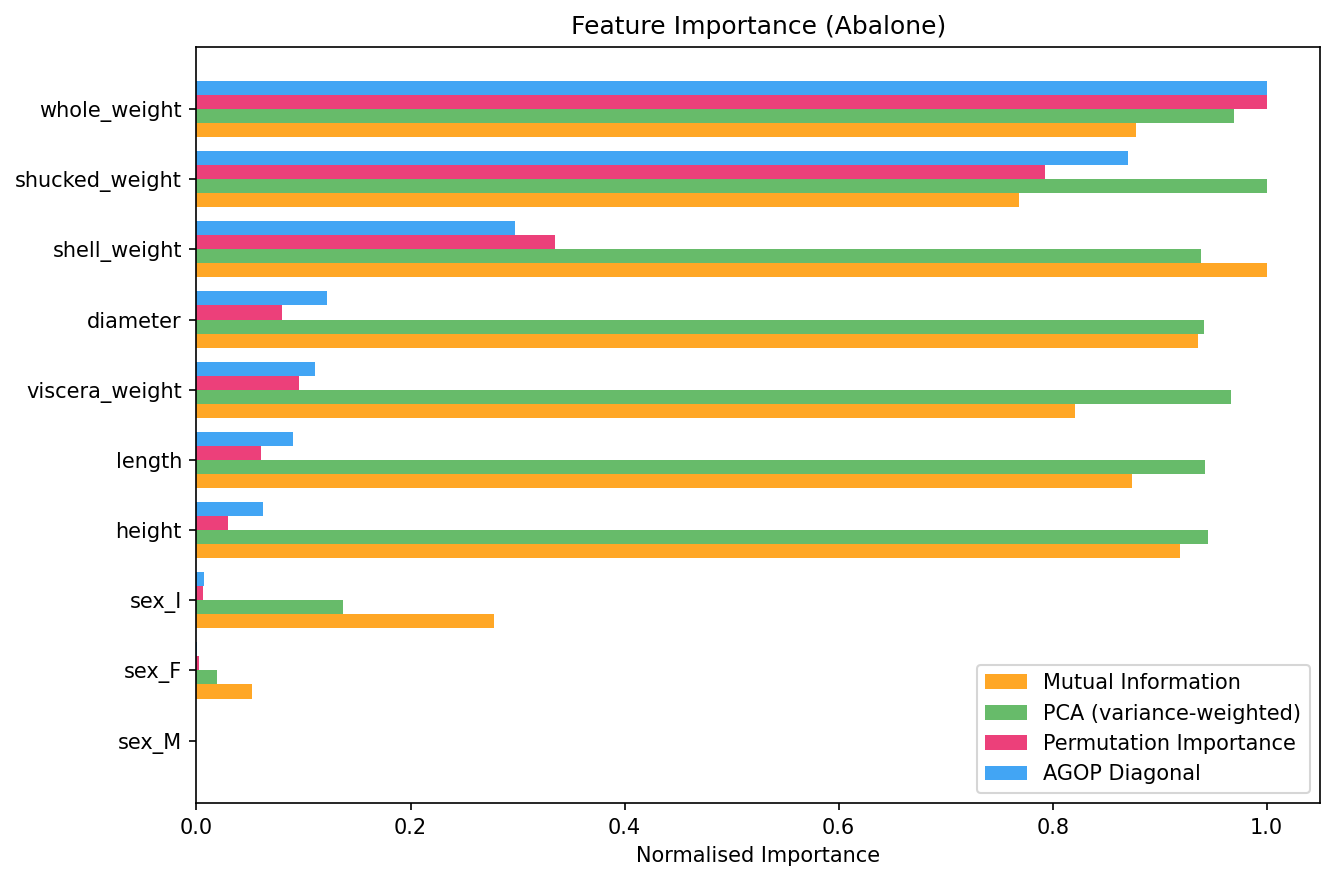
\includegraphics[width=\textwidth]{../results/03_interpretability/importance_bar.png}
    \caption{Normalised feature importance scores}
    \label{fig:interpretability_importance_bar}
  \end{subfigure}
  \hfill
  \begin{subfigure}[b]{0.49\textwidth}
    \centering
    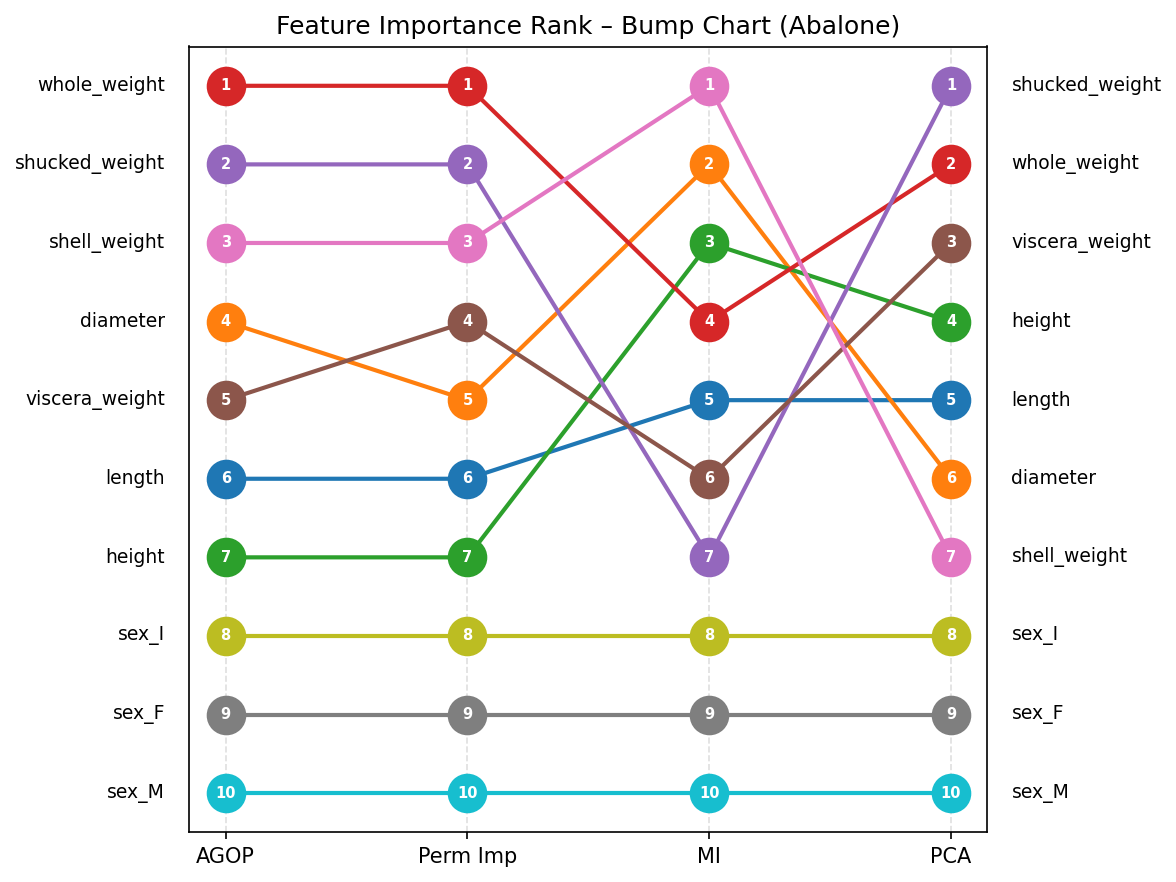
\includegraphics[width=\textwidth]{../results/03_interpretability/bump_chart.png}
    \caption{Rank comparison across methods}
    \label{fig:interpretability_bump_chart}
  \end{subfigure}
  \caption{Interpretability comparison on the Abalone dataset. We compare xRFM's AGOP-diagonal feature importances against PCA (variance-weighted loadings), mutual information, and permutation importance.}
  \label{fig:interpretability}
\end{figure}

\subsection{Scalability Analysis}
% On one large dataset (n > 10,000), subsample the training set at several sizes and plot test performance and training time versus n for all models.
\begin{figure}[H]
  \centering
  \begin{subfigure}[b]{0.32\textwidth}
    \centering
    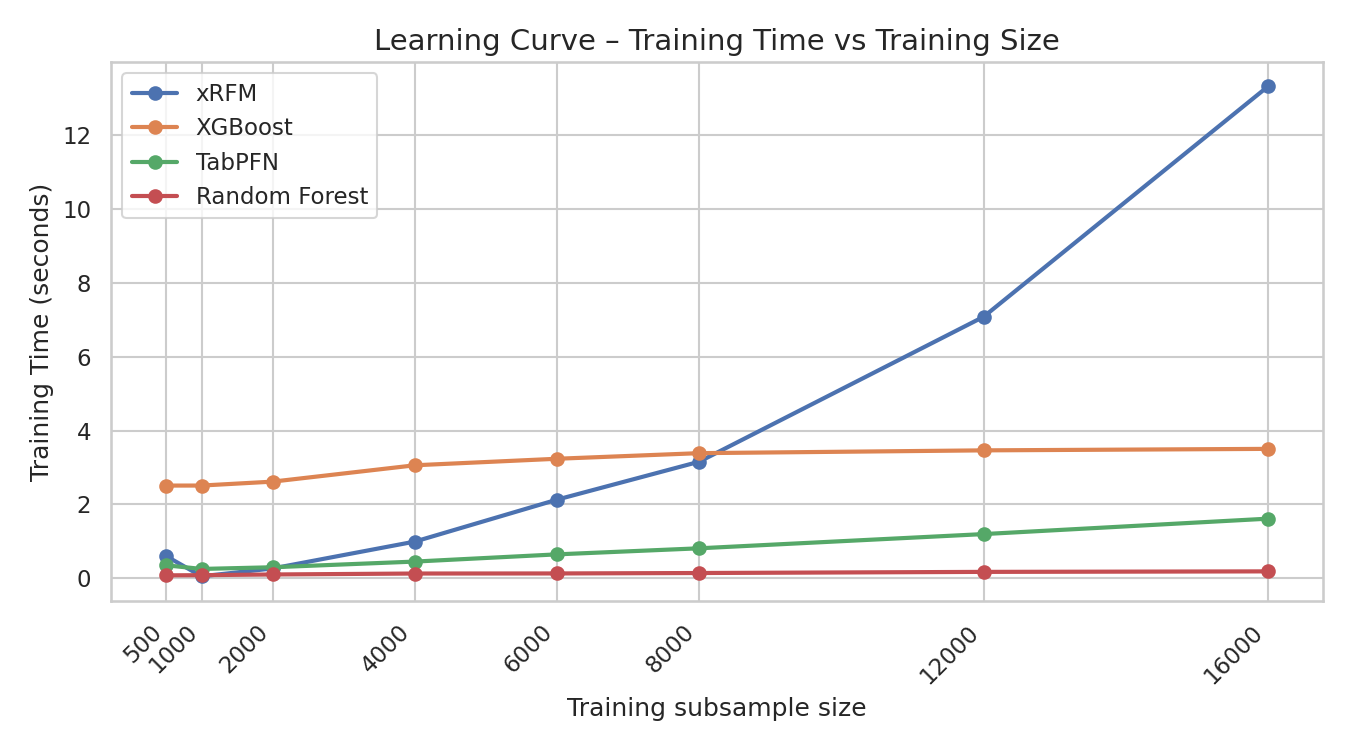
\includegraphics[width=\textwidth]{../results/04_learning_curve/learning_curve_sleep_health_fit_time.png}
    \caption{Training time}
    \label{fig:scalability_sleep_health_fit_time}
  \end{subfigure}
  \hfill
  \begin{subfigure}[b]{0.32\textwidth}
    \centering
    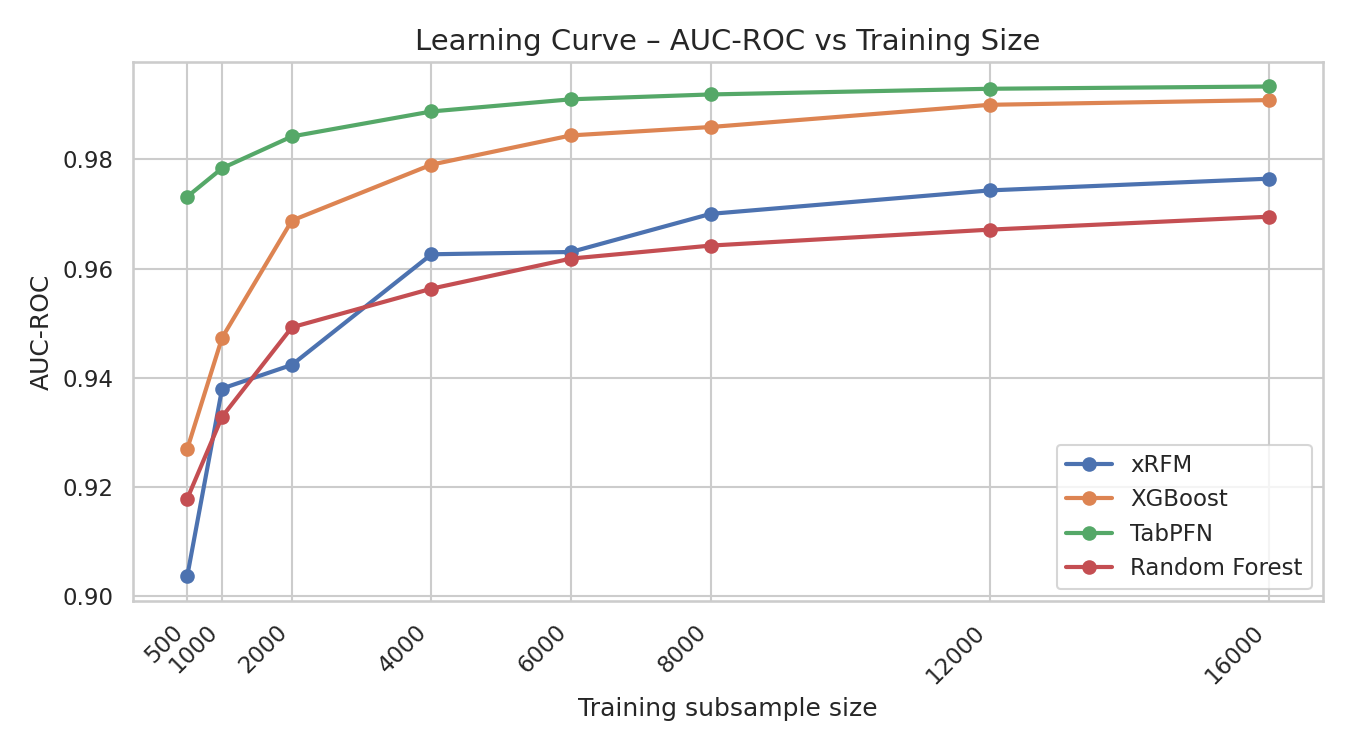
\includegraphics[width=\textwidth]{../results/04_learning_curve/learning_curve_sleep_health_auc_roc.png}
    \caption{AUC-ROC}
    \label{fig:scalability_sleep_health_auc_roc}
  \end{subfigure}
  \hfill
  \begin{subfigure}[b]{0.32\textwidth}
    \centering
    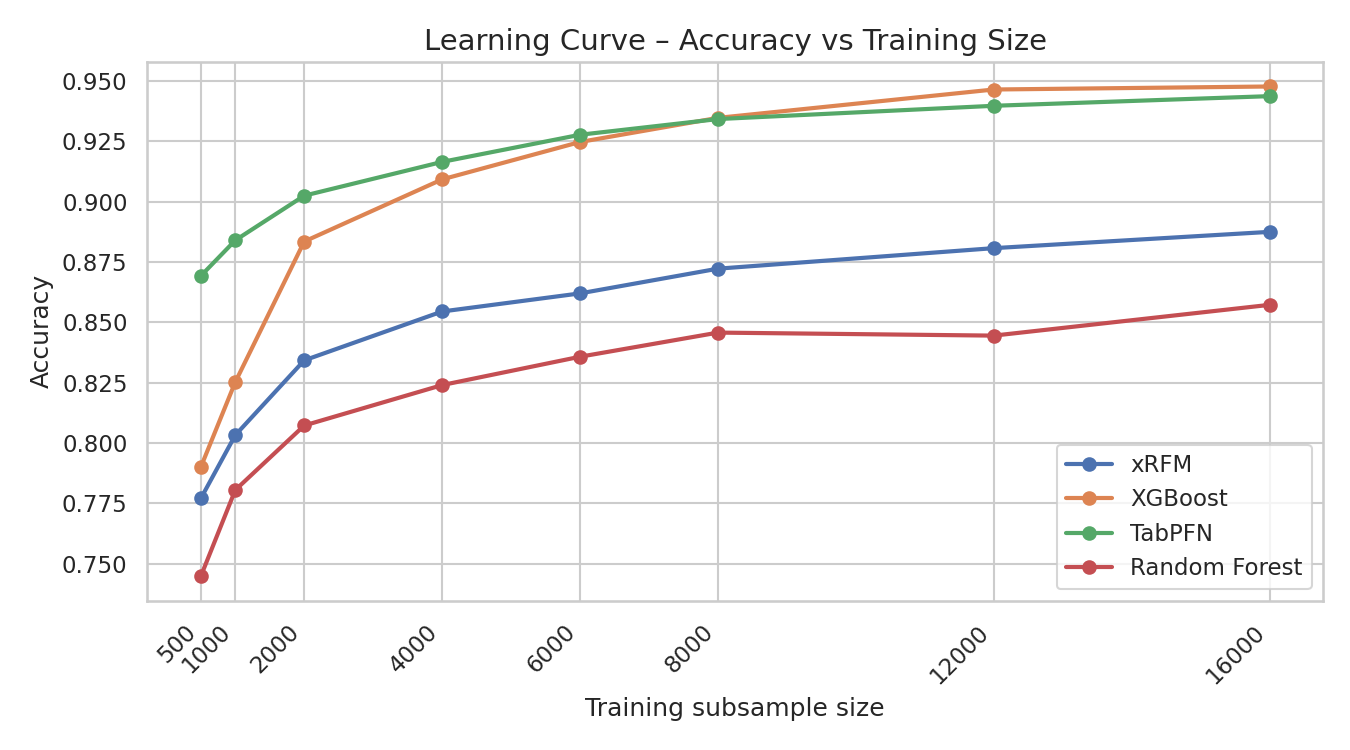
\includegraphics[width=\textwidth]{../results/04_learning_curve/learning_curve_sleep_health_accuracy.png}
    \caption{Accuracy}
    \label{fig:scalability_sleep_health_accuracy}
  \end{subfigure}
  \caption{Scalability analysis on the Sleep Health dataset (classification task; target: \texttt{sleep\_disorder\_risk}). We plot training time and test performance against the number of training samples $n$ for all models.}
  \label{fig:scalability}
\end{figure}

We evaluate scalability on the Sleep Health dataset, a multi-class classification task that predicts the \texttt{sleep\_disorder\_risk} label from mixed numerical and categorical features. As the training subsample size $n$ increases, we observe consistent improvements in predictive performance for all models in terms of both AUC-ROC and Accuracy, with gains diminishing as curves begin to saturate at larger $n$. In contrast, training time generally increases with $n$: xRFM exhibits the steepest growth in total training time as $n$ becomes large, while tree-based baselines (Random Forest and XGBoost) remain comparatively stable in this range, and TabPFN stays fast across all subsample sizes. Overall, these results highlight the expected trade-off between improved generalization from more data and the computational cost of training, and show that different model families scale quite differently on the same large tabular classification dataset.
